\section{Lec 17}
\subsection{Geodesic of Schwarzschild}
We derived the metric 
\[
ds^{2} = - \left( 1- \frac{2GM}{r} \right)dt^{2} + \left( 1- \frac{2GM}{r} \right)^{-1}dr^{2} + r^{2} d\Omega ^{2}
\]
now, the geodesic for test particles is
\[
\frac{d x^{2}}{d \lambda ^{2}} + \Gamma ^{\mu }_{\alpha \beta } \frac{d x^{\alpha }}{d \lambda }\frac{d x^{\beta }}{d \lambda } = 0
\]
In the Newtonian limit there are two quantities that are the \emph{effective potential}, that combines multiple effect into a single potential. It is defined as
\[
V_{eff}\left( r \right) = \frac{L^{2}}{2mr^{2}} - \frac{GMm}{r}
\]
where \emph{L} is the angular momentum, \emph{r} is the distance between the two masses, \emph{m} is the mass of the orbiting body and the second term is the potential.
There is the \emph{energy, E}
\[
	E = \frac{1}{2}m\dot{r}^{2} + V_{eff}\left( r \right)
\]
we said about geodesic that they're a trajectory that parallel transport  the momentum vector
\[
p^{\nu }\nabla _{\nu }p^{\mu } = 0
\]
lower one index, so
\[
p^{\nu }\nabla _{\nu }p_{\mu } = 0
\]
this is null also because of metric compatibility. I think this means that I can bring in the metric without spoiling the result. We remember that $p^{\nu } \equiv \frac{d x^{\nu }}{d \lambda }$.
The equation will go in this way
\begin{align}
	p^{\nu }\nabla _{\nu }p_{\mu } &= 0 \\
	p^{\nu }\left[ \partial_{\nu }p_{\mu } - \Gamma ^{\sigma }_{\nu \mu }p_{\sigma } \right] & = 0 \\
	\frac{d x^{\nu }}{d \lambda } \partial_{\nu }p_{\mu } &= \Gamma ^{\sigma }_{\nu \mu }p^{\nu }p_{\sigma } \\
	\frac{d x^{\nu }}{d \lambda }\frac{d }{d x^{ \nu }}p_{\mu } & = \Gamma ^{\sigma }_{\nu \mu }p^{\nu }p_{\sigma } \\
	\frac{d p_{\mu }}{d \lambda } &= \Gamma ^{\sigma }_{\nu \mu } p_{\sigma }p^{\nu }\\
	\frac{d p_{\mu }}{d \lambda } &= \frac{1}{2}g^{\sigma \rho } \left[ \partial_{\nu }g_{\rho \mu } + \partial_{\mu }g_{\rho \nu } - \partial_{\rho }g_{\mu \nu } \right] p_{\sigma }p^{\nu }
				      &= \frac{1}{2} p^{\nu }p^{\rho } \left[ \partial_{\mu }g_{\rho \nu } \right] \\
				     \frac{d p_{\mu }}{d \lambda } &= \frac{1}{2} \partial_{\mu }\left( g_{\rho \nu } \right) p^{\rho }p^{\nu } \\
\end{align}
What does it mean? Imagine there is a coordinate that does not appear in $g_{\mu \nu }$.
In fact looking at the expression of the metric at the start of the lecture, the metric does not explicitly depend on \emph{t}. This corresponds to the stationarity of the Schwarzschild spacetime. The conserved quantity associated with this symmetry is the particle's energy \emph{E} related to \emph{p\textsubscript{t}}.\par
Same for the azimuthal angle $\phi $, the metric does not explicitly depend on it. It correspond to the spherical symmetry of this spacetime, invariance under rotation around the central mass. The conserved quantity associated with this symmetry is $p_{\phi }$.\par
Still because of spherical symmetry we can focus on trajectories such that $\theta  = \frac{\pi }{2}$, without loss of generality.

\subsubsection{Gravitational Redshift}
We put ourselves on Earth, far away from $R_{S}$.
\bigskip

\tikzset{every picture/.style={line width=0.5pt}} %set default line width to 0.75pt

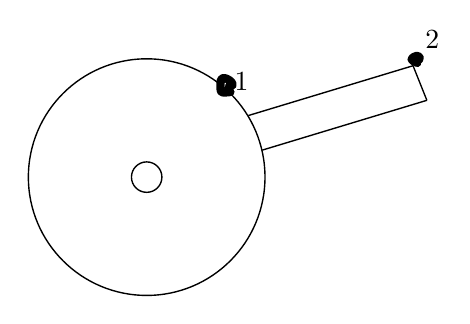
\begin{tikzpicture}[x=0.5pt,y=0.5pt,yscale=-1,xscale=1]
%uncomment if require: \path (0,300); %set diagram left start at 0, and has height of 300

%Shape: Circle [id:dp9321428345522449]
\draw   (240,154.5) .. controls (240,107.28) and (278.28,69) .. (325.5,69) .. controls (372.72,69) and (411,107.28) .. (411,154.5) .. controls (411,201.72) and (372.72,240) .. (325.5,240) .. controls (278.28,240) and (240,201.72) .. (240,154.5) -- cycle ;
%Shape: Circle [id:dp3143161131851636]
\draw   (314.5,154.5) .. controls (314.5,148.42) and (319.42,143.5) .. (325.5,143.5) .. controls (331.58,143.5) and (336.5,148.42) .. (336.5,154.5) .. controls (336.5,160.58) and (331.58,165.5) .. (325.5,165.5) .. controls (319.42,165.5) and (314.5,160.58) .. (314.5,154.5) -- cycle ;
%Straight Lines [id:da5051772731816909]
\draw    (409,135) -- (528,99) ;
%Straight Lines [id:da3890542297065277]
\draw    (399,110) -- (518,74) ;
%Straight Lines [id:da012166969683247708]
\draw    (518,74) -- (528,99) ;
%Shape: Free Drawing [id:dp5207276669171959]
\draw  [line width=3] [line join = round][line cap = round] (386,93) .. controls (383.64,93) and (379.29,94.34) .. (379,92) .. controls (378.71,89.68) and (378.71,87.32) .. (379,85) .. controls (379.8,78.56) and (393.19,89) .. (385,89) ;
%Shape: Free Drawing [id:dp028810113983297803]
\draw  [line width=3] [line join = round][line cap = round] (521,72) .. controls (521,71.41) and (514.41,70.15) .. (518,68) .. controls (524.18,64.29) and (523.85,71) .. (520,71) ;

% Text Node
\draw (387,77) node [anchor=north west][inner sep=0.75pt]   [align=left] {1};
% Text Node
\draw (525,47) node [anchor=north west][inner sep=0.75pt]   [align=left] {2};

\end{tikzpicture}
\bigskip
We emit a photon from the bottom to the top of the tower, of frequency $\nu $, we will find the relation between $\omega _{1}, \omega _{2}$.\par
This is a radial trajectory, this means that $d\phi =0$.
Now we will unravel the conserved quantity $p_{t}$
\begin{gather*}
	p_{t} = g_{t\alpha }p^{\alpha } = g_{tt} p^{t} \\
	p_{t} = - \left( 1- \frac{2GM}{r} \right) \frac{d t}{d \lambda } = \text{ const } = \alpha  
\end{gather*}
Now the goal is to find what $\omega _{1}$ is. I am sitting on 1. I want to achieve the first frequency $\omega _{1}$. In LIC we have
\begin{gather*}
u^{\hat{\mu }} = \left( 1,0,0,0 \right) \\
p^{\hat{\mu }} = \left( \omega , \omega \hat{n} \right)
\end{gather*}

The angular frequency is given by 
\[
\omega  = - u^{\hat{\mu }}p_{\hat{\mu }}
\]
but this has to be true in every coordinate system so
\[
\omega  = -u^{\mu }p_{\mu }
\]
Now, what we want is to know what is the angular frequency observed by observer.
He has four velocity 
\[
u^{\mu } = \left( 1,0,0,0 \right)
\]
and we know that 
\[
u^{\mu }u_{\mu } = -1
\]
since almost all the components are null we get the same writing
\[
g_{00}u^{0}u^{0} = -1
\]
and this leads us to find
\[
\omega = - g_{00}u^{0}p^{0} = \left( 1- \frac{2GM}{r} \right)\left( 1- \frac{2GM}{r} \right)^{-\frac{1}{2}} \frac{d t}{d \lambda } = \alpha \left( 1 - \frac{2GM}{r} \right)^{-\frac{1}{2}}
\]
so, as the photon moves radially, its energy will change.
\begin{equation}
\frac{\omega _{2}}{\omega _{1}} = \frac{\left( 1 - \frac{2GM}{r_{1}} \right)^{\frac{1}{2}}}{\left( 1- \frac{2GM}{r_{2}} \right)^{\frac{1}{2}}} \approx 1 - \frac{GM}{r_{1}} + \frac{GM}{r_{2}} = 1 - \Delta \phi 
\end{equation}
or 
\[
\frac{\Delta \omega }{\omega } = - \Delta \phi 
\]
where this $\phi $ is the gravitational potential, not a coordinate.


























